%\documentclass[11pt]{article}
\documentclass[answers]{exam}

\usepackage{amsmath}
%\usepackage{extsizes}
\usepackage{amsmath,amssymb}
%\usepackage{omegavn,ocmrvn}
%\usepackage[utf8x]{inputenc}
\usepackage[utf8]{vietnam}
\DeclareUnicodeCharacter{00A0}{ }

\usepackage{listings}
\lstset{language=Python}          % Set your language (you can change the language for each code-block optionally)

\usepackage{longtable}
\usepackage{answers}
\usepackage{graphicx}
\usepackage{array}
\usepackage{pifont}
\usepackage{picinpar}
\usepackage{enumerate}
\usepackage[top=3.0cm, bottom=3.5cm, left=3.5cm, right=2.5cm] {geometry}

\usepackage{hyperref}


\newtheorem{bt}{Câu}
\newcommand{\RR}{\mathbb R}
\Newassociation{sol}{Solution}{ans}
\newtheorem{ex}{Câu}
\renewcommand{\solutionstyle}[1]{\textbf{ #1}.}


\begin{document}
% \noindent
\begin{tabular*}
{\linewidth}{c>{\centering\hspace{0pt}} p{.7\textwidth}}
Trường ĐHKHTN, ĐHQGHN & {\bf Học Kỳ 1 (2021-2022)}
\tabularnewline
{K64 TTƯD - Lớp thầy Hà Phi} & {\bf Bài Tập Giải Tích Số. No 0 \\ \today}
\tabularnewline
\rule{1in}{1pt}  \small  & \rule{2in}{1pt} %(Due date:)
\tabularnewline

%  \tabularnewline
%  &(Đề thi có 1 trang)
\end{tabular*}
%
%\Opensolutionfile{ans}[ans1]
\printanswers

\begin{bt}\label{bt1}
Viết hàm trong Python để đổi độ F ra độ C (google cách đổi). Kiểm tra thử xem F = 69.8 thì C = 21 đúng không?
%Khi viết hàm phải có phần giải thích và ghi tên, ví dụ
%%
%\begin{lstlisting}[frame=single] 
%"""
%This is  a function to convert degree F to degree C
%Using the formula C = .....
%Name: Phi Ha, K64 TTUD/MT_KHTT
%"""
%
%def doi_nhiet_do(F):
%
%......
%
%return C
%\end{lstlisting}
%%
\end{bt}

\begin{bt} 
	Import hàm giai thừa trong module math sử dụng lệnh \verb| from math import factorial|. \\
	a) Hãy tính xấp xỉ $e$ sử dụng 1000 số hạng đầu tiên trong khai triển MacLaurin như sau
	%
	\[
	e = 1 + \sum_{k=1}^{1000} \dfrac{1}{k!} \ .
	\]
	%
	b) Hãy tính xấp xỉ $e$ chính xác đến 9 chữ số thập phân. Gợi ý sử dụng vòng lặp for và kiểm tra sai số 2 bước liên tiếp có $<= 1e-10$ không.
\end{bt}

\begin{bt} Ôn lại thuật toán Horner. \\
a) So sánh 2 cách tính toán hàm số $f(x) = 2x^2 + 3 x + 4$ dưới đây xem cách nào tiết kiệm thời gian hơn. Số flops của mỗi cách tính là bao nhiêu?
%
\begin{equation}
 \mbox{Cách 1: } \	value = 2 * x * x + 3 * x + 4 \quad  \mbox{Cách 2: } \	value = (2 * x + 3) * x + 4 \ .
\end{equation}
%
b) Từ câu a) hoặc google hãy tìm hiểu về thuật toán Horner và viết hàm theo $n$ để tính giá trị đa thức P(x) sau tại $x = 1.1$ một cách hiệu quả
%
\[
p(x) = (n+1) x^n + n x^{n-1} + ... + 2x + 1 \ .
\]
%
Số $n$ lớn nhất các em có thể tìm được là bao nhiêu (làm tròn đến 1000)? \\
c) Hãy viết hàm để tính giá trị đa thức $P(x)$ tại điểm $x_0$, với đầu vào input là $x_0$ và 1 vector hệ số (có độ dài bất kỳ) $a = [a_0 a_{1} ... a_{n}]$, $n = \deg(P)$. Hàm dạng như sau.

%
\begin{lstlisting}[frame=single] 
	"""
	This is  a function to compute the value P(x)
	Using Horner nested multiplication
	Name: Phi Ha, K64 TTUD/MT_KHTT
	"""
	
	def horner(a,x):
	
	......
	
	return value
\end{lstlisting}
%
\end{bt}


\begin{bt} Lực kéo trên một vật thể, theo sức cản không khí, được tính bởi  
%
\[
F_d = \dfrac{1}{2} C_D \rho A V^2, \\
\]
%
trong đó $\rho$ là mật độ của khí, V là vận tốc của vật thể, A là diện tích tiếp xúc 
(vuông góc với hướng vận tốc), và $C_D$ là hệ số kéo, phụ thuộc vào hình dạng của vật thể và độ gồ ghề của bề mặt vật thể đó. 
%
\begin{figure}[!h]
	\centering
	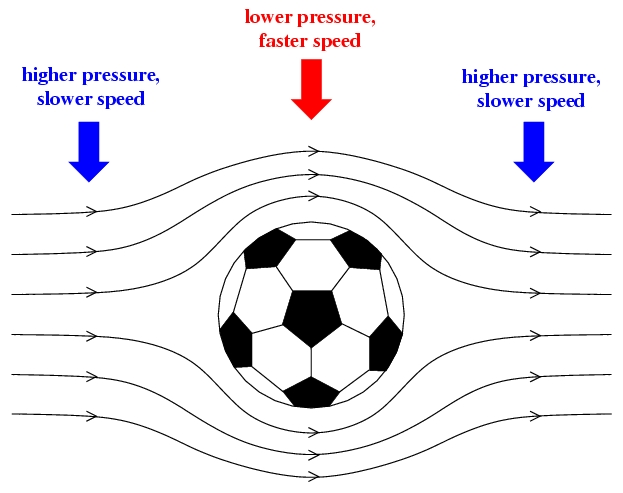
\includegraphics[width=0.7\linewidth]{forces_on_football}
	\caption{Tính toán lực cản của môi trường khí lên quả bóng đá. Source https://www.physics.hku.hk/~phys0607/lectures/chap05.html}
	\label{fig:forcesonfootball}
\end{figure}
%
Lực hấp dẫn trên một bề mặt với khối lượng $m$ là $F_g = mg$, trong đó $g = 9.81m s^{-2}$.
Chúng ta có thể dùng các công thức của $F_d$ và $F_g$ để nghiên cứu mức độ tác động của không khí và trọng lực khi đá một quả bóng. 
Mật độ không khí là $\rho = 1.2 kg/m^3$. 
$A = \pi a^2$ với mọi quả bóng mà bán kính là $a$. Thông thường với bóng đá $a = 11 cm$. 
Khối lượng quả bóng đá là $0.43 kg$, $C_D= 0.2$. 
Viết hàm tính toán các lực trên và in kết quả ra khi đá quả bóng với vận tốc $V = 120 km/h$ (mạnh) và $V = 10 km/h$ (yếu).
Đặc biệt chú ý đến đơn vị của V khi tính. Đặt tên hàm/file là \verb|kick|.
\end{bt}

\centerline{——————————— Bài Tập Tự Luyện  ——————————}

\begin{bt}
	Convert from meters to British length units. Make a program where you set a length given in meters and then
	compute and write out the corresponding length measured in inches, in feet, in yards, and in miles. Use that one inch is 2.54 cm, one foot is
	12 inches, one yard is 3 feet, and one British mile is 1760 yards. As a verification, a length of 640 meters corresponds to 25196.85 inches,
	2099.74 feet, 699.91 yards, or 0.3977 miles. Name of program file: \verb|length_conversion.py| or the function \verb|length_conversion|. 
\end{bt}


\begin{bt} Compute the growth of money in a bank. \\
	Let $p$ be a bank’s interest rate in percent per year. An initial amount A has then grown to $A \ \left(1 + \dfrac{p}{100}\right)^n$
	after $n$ years. Make a program for computing how much money 1000 euros have grown to after three years with 5\% interest rate. Name of
	program file: \verb|interest_rate.py|. 
\end{bt}

\centerline{———————————Hết——————————}


%\vspace{1cm}
%\noindent{\bf Chú ý:} {\it Cán bộ coi thi không giải thích gì thêm}\\
%\vspace{0.4cm}
%\noindent{\bf Họ và tên học sinh: \rule{3in}{.01pt} Lớp: \hrulefill}
%\Closesolutionfile{ans}
%\newpage
%\begin{center}
%{\LARGE{\bf ĐÁP ÁN}}
%\end{center}
%\begin{Solution}{1}
	\begin{figure}[h!]
		\centering
		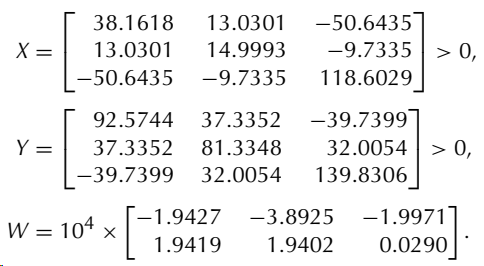
\includegraphics[width=0.7\linewidth]{Solution1/screenshot001}
		\caption[Exercise 1.2.5, Burden-Faires, 8ed.]{}
		\caption{}
		\label{fig:screenshot001}
	\end{figure}
\end{Solution}
 
   
\end{document}